\documentclass[]{book}
\usepackage{lmodern}
\usepackage{amssymb,amsmath}
\usepackage{ifxetex,ifluatex}
\usepackage{fixltx2e} % provides \textsubscript
\ifnum 0\ifxetex 1\fi\ifluatex 1\fi=0 % if pdftex
  \usepackage[T1]{fontenc}
  \usepackage[utf8]{inputenc}
\else % if luatex or xelatex
  \ifxetex
    \usepackage{mathspec}
  \else
    \usepackage{fontspec}
  \fi
  \defaultfontfeatures{Ligatures=TeX,Scale=MatchLowercase}
\fi
% use upquote if available, for straight quotes in verbatim environments
\IfFileExists{upquote.sty}{\usepackage{upquote}}{}
% use microtype if available
\IfFileExists{microtype.sty}{%
\usepackage{microtype}
\UseMicrotypeSet[protrusion]{basicmath} % disable protrusion for tt fonts
}{}
\usepackage[margin=1in]{geometry}
\usepackage{hyperref}
\hypersetup{unicode=true,
            pdftitle={Notes on Biostatistics},
            pdfauthor={Phùng Khánh Lâm},
            pdfborder={0 0 0},
            breaklinks=true}
\urlstyle{same}  % don't use monospace font for urls
\usepackage{natbib}
\bibliographystyle{apalike}
\usepackage{color}
\usepackage{fancyvrb}
\newcommand{\VerbBar}{|}
\newcommand{\VERB}{\Verb[commandchars=\\\{\}]}
\DefineVerbatimEnvironment{Highlighting}{Verbatim}{commandchars=\\\{\}}
% Add ',fontsize=\small' for more characters per line
\usepackage{framed}
\definecolor{shadecolor}{RGB}{248,248,248}
\newenvironment{Shaded}{\begin{snugshade}}{\end{snugshade}}
\newcommand{\AlertTok}[1]{\textcolor[rgb]{0.94,0.16,0.16}{#1}}
\newcommand{\AnnotationTok}[1]{\textcolor[rgb]{0.56,0.35,0.01}{\textbf{\textit{#1}}}}
\newcommand{\AttributeTok}[1]{\textcolor[rgb]{0.77,0.63,0.00}{#1}}
\newcommand{\BaseNTok}[1]{\textcolor[rgb]{0.00,0.00,0.81}{#1}}
\newcommand{\BuiltInTok}[1]{#1}
\newcommand{\CharTok}[1]{\textcolor[rgb]{0.31,0.60,0.02}{#1}}
\newcommand{\CommentTok}[1]{\textcolor[rgb]{0.56,0.35,0.01}{\textit{#1}}}
\newcommand{\CommentVarTok}[1]{\textcolor[rgb]{0.56,0.35,0.01}{\textbf{\textit{#1}}}}
\newcommand{\ConstantTok}[1]{\textcolor[rgb]{0.00,0.00,0.00}{#1}}
\newcommand{\ControlFlowTok}[1]{\textcolor[rgb]{0.13,0.29,0.53}{\textbf{#1}}}
\newcommand{\DataTypeTok}[1]{\textcolor[rgb]{0.13,0.29,0.53}{#1}}
\newcommand{\DecValTok}[1]{\textcolor[rgb]{0.00,0.00,0.81}{#1}}
\newcommand{\DocumentationTok}[1]{\textcolor[rgb]{0.56,0.35,0.01}{\textbf{\textit{#1}}}}
\newcommand{\ErrorTok}[1]{\textcolor[rgb]{0.64,0.00,0.00}{\textbf{#1}}}
\newcommand{\ExtensionTok}[1]{#1}
\newcommand{\FloatTok}[1]{\textcolor[rgb]{0.00,0.00,0.81}{#1}}
\newcommand{\FunctionTok}[1]{\textcolor[rgb]{0.00,0.00,0.00}{#1}}
\newcommand{\ImportTok}[1]{#1}
\newcommand{\InformationTok}[1]{\textcolor[rgb]{0.56,0.35,0.01}{\textbf{\textit{#1}}}}
\newcommand{\KeywordTok}[1]{\textcolor[rgb]{0.13,0.29,0.53}{\textbf{#1}}}
\newcommand{\NormalTok}[1]{#1}
\newcommand{\OperatorTok}[1]{\textcolor[rgb]{0.81,0.36,0.00}{\textbf{#1}}}
\newcommand{\OtherTok}[1]{\textcolor[rgb]{0.56,0.35,0.01}{#1}}
\newcommand{\PreprocessorTok}[1]{\textcolor[rgb]{0.56,0.35,0.01}{\textit{#1}}}
\newcommand{\RegionMarkerTok}[1]{#1}
\newcommand{\SpecialCharTok}[1]{\textcolor[rgb]{0.00,0.00,0.00}{#1}}
\newcommand{\SpecialStringTok}[1]{\textcolor[rgb]{0.31,0.60,0.02}{#1}}
\newcommand{\StringTok}[1]{\textcolor[rgb]{0.31,0.60,0.02}{#1}}
\newcommand{\VariableTok}[1]{\textcolor[rgb]{0.00,0.00,0.00}{#1}}
\newcommand{\VerbatimStringTok}[1]{\textcolor[rgb]{0.31,0.60,0.02}{#1}}
\newcommand{\WarningTok}[1]{\textcolor[rgb]{0.56,0.35,0.01}{\textbf{\textit{#1}}}}
\usepackage{longtable,booktabs}
\usepackage{graphicx,grffile}
\makeatletter
\def\maxwidth{\ifdim\Gin@nat@width>\linewidth\linewidth\else\Gin@nat@width\fi}
\def\maxheight{\ifdim\Gin@nat@height>\textheight\textheight\else\Gin@nat@height\fi}
\makeatother
% Scale images if necessary, so that they will not overflow the page
% margins by default, and it is still possible to overwrite the defaults
% using explicit options in \includegraphics[width, height, ...]{}
\setkeys{Gin}{width=\maxwidth,height=\maxheight,keepaspectratio}
\IfFileExists{parskip.sty}{%
\usepackage{parskip}
}{% else
\setlength{\parindent}{0pt}
\setlength{\parskip}{6pt plus 2pt minus 1pt}
}
\setlength{\emergencystretch}{3em}  % prevent overfull lines
\providecommand{\tightlist}{%
  \setlength{\itemsep}{0pt}\setlength{\parskip}{0pt}}
\setcounter{secnumdepth}{5}
% Redefines (sub)paragraphs to behave more like sections
\ifx\paragraph\undefined\else
\let\oldparagraph\paragraph
\renewcommand{\paragraph}[1]{\oldparagraph{#1}\mbox{}}
\fi
\ifx\subparagraph\undefined\else
\let\oldsubparagraph\subparagraph
\renewcommand{\subparagraph}[1]{\oldsubparagraph{#1}\mbox{}}
\fi

%%% Use protect on footnotes to avoid problems with footnotes in titles
\let\rmarkdownfootnote\footnote%
\def\footnote{\protect\rmarkdownfootnote}

%%% Change title format to be more compact
\usepackage{titling}

% Create subtitle command for use in maketitle
\providecommand{\subtitle}[1]{
  \posttitle{
    \begin{center}\large#1\end{center}
    }
}

\setlength{\droptitle}{-2em}

  \title{Notes on Biostatistics}
    \pretitle{\vspace{\droptitle}\centering\huge}
  \posttitle{\par}
    \author{Phùng Khánh Lâm}
    \preauthor{\centering\large\emph}
  \postauthor{\par}
      \predate{\centering\large\emph}
  \postdate{\par}
    \date{2019-11-10}

\usepackage{booktabs}
\usepackage{amsthm}
\makeatletter
\def\thm@space@setup{%
  \thm@preskip=8pt plus 2pt minus 4pt
  \thm@postskip=\thm@preskip
}
\makeatother

\begin{document}
\maketitle

{
\setcounter{tocdepth}{1}
\tableofcontents
}
\hypertarget{preface}{%
\chapter*{Preface}\label{preface}}
\addcontentsline{toc}{chapter}{Preface}

\hypertarget{bookdown}{%
\chapter*{Bookdown}\label{bookdown}}
\addcontentsline{toc}{chapter}{Bookdown}

This is a \emph{sample} book written in \textbf{Markdown}. You can use anything that Pandoc's Markdown supports, e.g., a math equation \(a^2 + b^2 = c^2\).

The \textbf{bookdown} package can be installed from CRAN or Github:

\begin{Shaded}
\begin{Highlighting}[]
\KeywordTok{install.packages}\NormalTok{(}\StringTok{"bookdown"}\NormalTok{)}
\CommentTok{# or the development version}
\CommentTok{# devtools::install_github("rstudio/bookdown")}
\end{Highlighting}
\end{Shaded}

Remember each Rmd file contains one and only one chapter, and a chapter is defined by the first-level heading \texttt{\#}.

To compile this example to PDF, you need XeLaTeX. You are recommended to install TinyTeX (which includes XeLaTeX): \url{https://yihui.name/tinytex/}.

You can label chapter and section titles using \texttt{\{\#label\}} after them, e.g., we can reference Chapter \ref{intro}. If you do not manually label them, there will be automatic labels anyway, e.g., Chapter \ref{methods}.

Figures and tables with captions will be placed in \texttt{figure} and \texttt{table} environments, respectively.

\begin{Shaded}
\begin{Highlighting}[]
\KeywordTok{par}\NormalTok{(}\DataTypeTok{mar =} \KeywordTok{c}\NormalTok{(}\DecValTok{4}\NormalTok{, }\DecValTok{4}\NormalTok{, }\FloatTok{.1}\NormalTok{, }\FloatTok{.1}\NormalTok{))}
\KeywordTok{plot}\NormalTok{(pressure, }\DataTypeTok{type =} \StringTok{'b'}\NormalTok{, }\DataTypeTok{pch =} \DecValTok{19}\NormalTok{)}
\end{Highlighting}
\end{Shaded}

\begin{figure}

{\centering 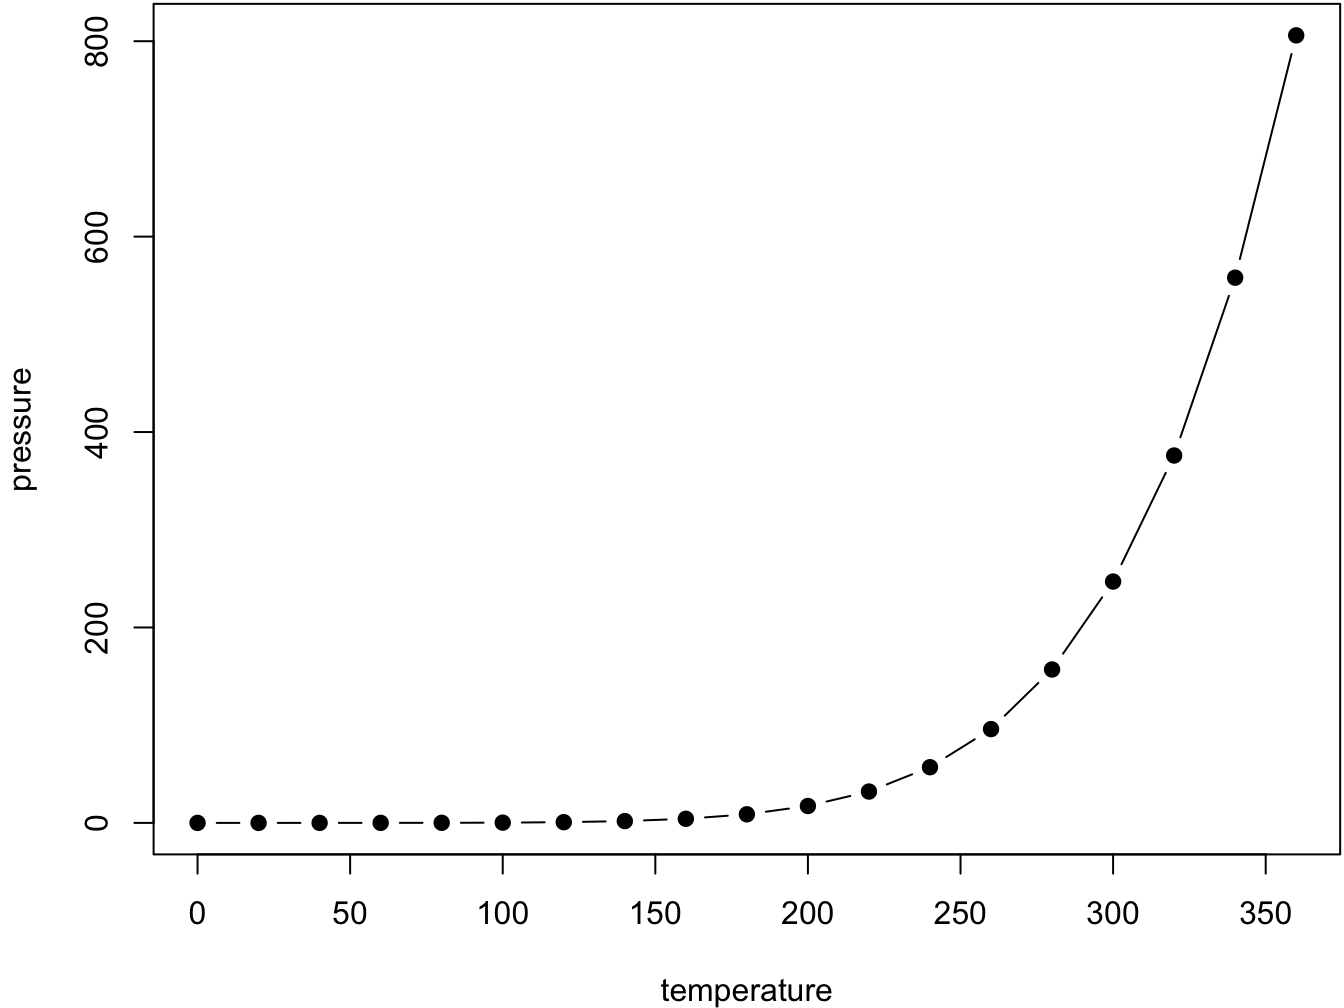
\includegraphics[width=0.8\linewidth]{notebook_Biostatistics_files/figure-latex/nice-fig-1} 

}

\caption{Here is a nice figure!}\label{fig:nice-fig}
\end{figure}

Reference a figure by its code chunk label with the \texttt{fig:} prefix, e.g., see Figure \ref{fig:nice-fig}. Similarly, you can reference tables generated from \texttt{knitr::kable()}, e.g., see Table \ref{tab:nice-tab}.

\begin{Shaded}
\begin{Highlighting}[]
\NormalTok{knitr}\OperatorTok{::}\KeywordTok{kable}\NormalTok{(}
  \KeywordTok{head}\NormalTok{(iris, }\DecValTok{20}\NormalTok{), }\DataTypeTok{caption =} \StringTok{'Here is a nice table!'}\NormalTok{,}
  \DataTypeTok{booktabs =} \OtherTok{TRUE}
\NormalTok{)}
\end{Highlighting}
\end{Shaded}

\begin{table}[t]

\caption{\label{tab:nice-tab}Here is a nice table!}
\centering
\begin{tabular}{rrrrl}
\toprule
Sepal.Length & Sepal.Width & Petal.Length & Petal.Width & Species\\
\midrule
5.1 & 3.5 & 1.4 & 0.2 & setosa\\
4.9 & 3.0 & 1.4 & 0.2 & setosa\\
4.7 & 3.2 & 1.3 & 0.2 & setosa\\
4.6 & 3.1 & 1.5 & 0.2 & setosa\\
5.0 & 3.6 & 1.4 & 0.2 & setosa\\
\addlinespace
5.4 & 3.9 & 1.7 & 0.4 & setosa\\
4.6 & 3.4 & 1.4 & 0.3 & setosa\\
5.0 & 3.4 & 1.5 & 0.2 & setosa\\
4.4 & 2.9 & 1.4 & 0.2 & setosa\\
4.9 & 3.1 & 1.5 & 0.1 & setosa\\
\addlinespace
5.4 & 3.7 & 1.5 & 0.2 & setosa\\
4.8 & 3.4 & 1.6 & 0.2 & setosa\\
4.8 & 3.0 & 1.4 & 0.1 & setosa\\
4.3 & 3.0 & 1.1 & 0.1 & setosa\\
5.8 & 4.0 & 1.2 & 0.2 & setosa\\
\addlinespace
5.7 & 4.4 & 1.5 & 0.4 & setosa\\
5.4 & 3.9 & 1.3 & 0.4 & setosa\\
5.1 & 3.5 & 1.4 & 0.3 & setosa\\
5.7 & 3.8 & 1.7 & 0.3 & setosa\\
5.1 & 3.8 & 1.5 & 0.3 & setosa\\
\bottomrule
\end{tabular}
\end{table}

You can write citations, too. For example, we are using the \textbf{bookdown} package \citep{R-bookdown} in this sample book, which was built on top of R Markdown and \textbf{knitr} \citep{xie2015}.

\hypertarget{new}{%
\chapter{New}\label{new}}

\begin{itemize}
\item
  Bianchi, M. T., Alexander, B. M., \& Cash, S. S. (2009). Incorporating Uncertainty Into Medical Decision Making: An Approach to Unexpected Test Results. Medical Decision Making, 29(1), 116--124. \url{https://doi.org/10.1177/0272989X08323620}
\item
  Nobles AL, Leas EC, Althouse BM, et al.~Requests for Diagnoses of Sexually Transmitted Diseases on a Social Media Platform. JAMA. 2019;322(17):1712--1713. \url{doi:https://doi.org/10.1001/jama.2019.14390}
\item
  Steve Ruberg (2019) No.~13: Unconsciously Biased and Consciously Unbiased. \url{https://analytixthinking.blog/2019/11/07/no-13-unconsciously-biased-and-consciously-unbiased/}
\item
  renv: Project Environments for R. \url{https://blog.rstudio.com/2019/11/06/renv-project-environments-for-r/}
\item
  The frontier of simulation-based inference. \url{https://deepai.org/publication/the-frontier-of-simulation-based-inference}
\item
  Non-randomized studies using causal-modelling may give different answers than RCTs: a meta-epidemiological study. DOI: \url{https://doi.org/10.1016/j.jclinepi.2019.10.012}.
\item
  Four mistakes to avoid when talking with patients about risk. \url{https://www.aafp.org/journals/fpm/blogs/inpractice/entry/risk_communication_mistakes.html\#.XDYKYKwH6CA.twitter}
\item
  5 mistakes of communicating risk. \url{https://www.youtube.com/watch?v=jAY3H92MXGU}
\item
  \citet{BenVanCalster}'s keynote on Machine learning: calm down!. \url{https://twitter.com/Georg__Heinze/status/1192796427619065857}
\item
  What logic gives us the authority to say something about an individual by observing other individuals, however similar? \url{https://twitter.com/yudapearl/status/1192768005316341760}. \url{http://ftp.cs.ucla.edu/pub/stat_ser/r375-reprint.pdf}
\item
  Just released today, and it is shameful: \url{https://ncd.gov/sites/default/files/NCD_Quality_Adjusted_Life_Report_508.pdf}. Recommendation against QALYs and \#healtheconomics to support resource allocation decisions. \url{https://twitter.com/dollendorf/status/1192181668985102338}
\item
  stats might kill personalized medicine. \url{https://twitter.com/KertViele/status/1192194206049226754}
\item
  RStudio Package Manager. \url{https://blog.rstudio.com/2019/11/07/package-manager-v1-1-no-interruptions/}
\end{itemize}

\hypertarget{ida}{%
\chapter{Initial data analysis}\label{ida}}

\hypertarget{DataCleaning}{%
\chapter{Data cleaning}\label{DataCleaning}}

\hypertarget{DescriptiveAnalysis}{%
\chapter{Descriptive analysis}\label{DescriptiveAnalysis}}

\hypertarget{graphics}{%
\chapter{Graphics}\label{graphics}}

\hypertarget{CausalInference}{%
\chapter{Causal Inference}\label{CausalInference}}

\hypertarget{reading-list}{%
\section{Reading list}\label{reading-list}}

\begin{itemize}
\tightlist
\item
  Daniel Westreich (2019) Epidemiology by Design: A Causal Approach to the Health Sciences. Oxford University Press. \url{https://global.oup.com/academic/product/epidemiology-by-design-9780190665760?cc=vn\&lang=en\&}
\end{itemize}

\hypertarget{StudyDesign}{%
\chapter{Study design}\label{StudyDesign}}

\hypertarget{HypothesisTesting}{%
\chapter{Hypothesis Testing}\label{HypothesisTesting}}

\hypertarget{Pvalue}{%
\chapter{P value}\label{Pvalue}}

\hypertarget{Bayesian}{%
\chapter{Bayesian data analysis}\label{Bayesian}}

\hypertarget{PredictionModels}{%
\chapter{Prediction models}\label{PredictionModels}}

\hypertarget{mdm}{%
\chapter{Medical decision making}\label{mdm}}

\hypertarget{reading-list-1}{%
\section{Reading list}\label{reading-list-1}}

\hypertarget{risk-communication}{%
\subsection{Risk communication}\label{risk-communication}}

\begin{itemize}
\item
  Sisk BA, Baker JN (2018) Microethics of Communication---Hidden Roles of Bias and Heuristics in the Words We Choose. JAMA Pediatr;172(12):1115--1116. \url{doi:https://doi.org/10.1001/jamapediatrics.2018.3111}.
\item
  Steinhardt Joe (2019) The role of numeric and statistical content on risk perception in infographics about road safety, Journal of Risk Research, \url{DOI:10.1080/13669877.2019.1596147}
\item
  Kunneman M, Stiggelbout AM, Pieterse AH (2019) Do clinicians convey what they intend? Lay interpretation of verbal risk labels used in decision encounters. Patient Educ Couns. 2019 Aug 26. pii: S0738-3991(19)30377-5. doi: 10.1016/j.pec.2019.08.035.
\item
  NICE guidance on risk communication: \url{https://twitter.com/BerksMaternity/status/1171542152842817536/photo/1}. \href{figures/mdm/nicenice_riskcommunication.jpeg}{Figure}
\item
  Okan Y, Smith SG, Bruine de Bruin W (2019) How is cervical cancer screening information communicated in UK websites? Cross-sectional analysis of content and quantitative presentation formatsBMJ Open 2019;9:e029551. doi: 10.1136/bmjopen-2019-029551.
\item
  Yen, Renata W, Barr, Paul J, Cochran, Nan, Aarts, Johanna W, Légaré, France, Reed, Malcolm, O'Mallley, A James, Scalia, Peter, Guérard, Genevieve Painchaud, Backer, Grant, Reilly, Clifford, Elwyn, Glyn and Durand, Marie-Anne (2019) Medical students' knowledge and attitudes towards shared decision-making: results from a multinational cross-sectional survey. Medical Decision Making. \url{http://sro.sussex.ac.uk/id/eprint/85728/}
\item
\end{itemize}

\hypertarget{ild}{%
\chapter{Intensive Longitudinal data analysis}\label{ild}}

\hypertarget{reading-list-2}{%
\section{Reading list}\label{reading-list-2}}

\hypertarget{papers}{%
\subsection{Papers:}\label{papers}}

\begin{itemize}
\item
  T. Asparouhov, E. L. Hamaker, and B. Muthén. ``Dynamic Structural Equation Models''. In: \emph{Structural Equation Modeling:
  A Multidisciplinary Journal} 25.3 (Dec.~2017), pp.~359-388. DOI: 10.1080/10705511.2017.1406803. \textless{}URL:
  \url{https://doi.org/10.1080/10705511.2017.1406803}\textgreater{}.
\item
  T. Asparouhov and B. Muthén. ``Comparison of Models for the Analysis of Intensive Longitudinal Data''. In: \emph{Structural
  Equation Modeling: A Multidisciplinary Journal} (Jul.~2019), pp.~1-23. DOI: 10.1080/10705511.2019.1626733. \textless{}URL:
  \url{https://doi.org/10.1080/10705511.2019.1626733}\textgreater{}.
\item
  E. M. Chi and G. C. Reinsel. ``Models for Longitudinal Data with Random Effects and AR(1) Errors''. In: \emph{Journal of the
  American Statistical Association} 84.406 (Jun.~1989), pp.~452-459. DOI: 10.1080/01621459.1989.10478790. \textless{}URL:
  \url{https://doi.org/10.1080/01621459.1989.10478790}\textgreater{}.
\item
  L. M. Collins. ``Analysis of Longitudinal Data: The Integration of Theoretical Model, Temporal Design, and Statistical
  Model''. In: \emph{Annual Review of Psychology} 57.1 (Jan.~2006), pp.~505-528. DOI: 10.1146/annurev.psych.57.102904.190146.
  \textless{}URL: \url{https://doi.org/10.1146/annurev.psych.57.102904.190146}\textgreater{}.
\item
  S. C. Duncan, T. E. Duncan, and H. Hops. ``Analysis of longitudinal data within accelerated longitudinal designs.'' In:
  \emph{Psychological Methods} 1.3 (1996), pp.~236-248. DOI: 10.1037/1082-989x.1.3.236. \textless{}URL:
  \url{https://doi.org/10.1037/1082-989x.1.3.236}\textgreater{}.
\item
  T. E. Duncan and S. C. Duncan. ``An introduction to latent growth curve modeling''. In: \emph{Behavior Therapy} 35.2 (2004),
  pp.~333-363. DOI: 10.1016/s0005-7894(04)80042-x. \textless{}URL: \url{https://doi.org/10.1016/s0005-7894(04)80042-x}\textgreater{}.
\item
  E. L. Hamaker and M. Wichers. ``No Time Like the Present''. In: \emph{Current Directions in Psychological Science} 26.1
  (Feb.~2017), pp.~10-15. DOI: 10.1177/0963721416666518. \textless{}URL: \url{https://doi.org/10.1177/0963721416666518}\textgreater{}.
\item
  E. L. Hamaker, T. Asparouhov, A. Brose, et al. ``At the Frontiers of Modeling Intensive Longitudinal Data: Dynamic
  Structural Equation Models for the Affective Measurements from the COGITO Study''. In: \emph{Multivariate Behavioral Research}
  53.6 (Apr.~2018), pp.~820-841. DOI: 10.1080/00273171.2018.1446819. \textless{}URL: \url{https://doi.org/10.1080/00273171.2018.1446819}\textgreater{}.
\item
  N. C. Jacobson, S. Chow, and M. G. Newman. ``The Differential Time-Varying Effect Model (DTVEM): A tool for diagnosing
  and modeling time lags in intensive longitudinal data''. In: \emph{Behavior Research Methods} 51.1 (Aug.~2018), pp.~295-315.
  DOI: 10.3758/s13428-018-1101-0. \textless{}URL: \url{https://doi.org/10.3758/s13428-018-1101-0}\textgreater{}.
\item
  S. Jahng and P. K. Wood. ``Multilevel Models for Intensive Longitudinal Data with Heterogeneous Autoregressive Errors:
  The Effect of Misspecification and Correction with Cholesky Transformation''. In: \emph{Frontiers in Psychology} 8 (Feb.~2017).
  DOI: 10.3389/fpsyg.2017.00262. \textless{}URL: \url{https://doi.org/10.3389/fpsyg.2017.00262}\textgreater{}.
\item
  M. Karas, J. Bai, M. Strączkiewicz, et al. ``Accelerometry Data in Health Research: Challenges and Opportunities''.
  In: \emph{Statistics in Biosciences} 11.2 (Jan.~2019), pp.~210-237. DOI: 10.1007/s12561-018-9227-2. \textless{}URL:
  \url{https://doi.org/10.1007/s12561-018-9227-2}\textgreater{}.
\item
  S. T. Lanza, S. A. Vasilenko, and M. A. Russell. ``Time-varying effect modeling to address new questions in
  behavioral research: Examples in marijuana use.'' In: \emph{Psychology of Addictive Behaviors} 30.8 (Dec.~2016), pp.~939-954.
  DOI: 10.1037/adb0000208. \textless{}URL: \url{https://doi.org/10.1037/adb0000208}\textgreater{}.
\item
  Y. Miyazaki and S. W. Raudenbush. ``Tests for linkage of multiple cohorts in an accelerated longitudinal design.'' In:
  \emph{Psychological Methods} 5.1 (2000), pp.~44-63. DOI: 10.1037/1082-989x.5.1.44. \textless{}URL:
  \url{https://doi.org/10.1037/1082-989x.5.1.44}\textgreater{}.
\item
  S. W. RAUDENBUSH and W. CHAN. ``Growth Curve Analysis in Accelerated Longitudinal Designs''. In: \emph{Journal of Research
  in Crime and Delinquency} 29.4 (Nov.~1992), pp.~387-411. DOI: 10.1177/0022427892029004001. \textless{}URL:
  \url{https://doi.org/10.1177/0022427892029004001}\textgreater{}.
\item
  J. Windt, C. L. Ardern, T. J. Gabbett, et al. ``Getting the most out of intensive longitudinal data: a methodological
  review of workload\textendashinjury studies''. In: \emph{BMJ Open} 8.10 (Oct.~2018), p.~e022626. DOI:
  10.1136/bmjopen-2018-022626. \textless{}URL: \url{https://doi.org/10.1136/bmjopen-2018-022626}\textgreater{}.
\item
  S. Yang, J. A. Cranford, R. Li, et al. ``A time-varying effect model for studying gender differences in health
  behavior''. In: \emph{Statistical Methods in Medical Research} 26.6 (Oct.~2015), pp.~2812-2820. DOI: 10.1177/0962280215610608.
  \textless{}URL: \url{https://doi.org/10.1177/0962280215610608}\textgreater{}.
\end{itemize}

\hypertarget{books}{%
\subsection{Books}\label{books}}

\begin{itemize}
\item
  Walls T, Schafer J (eds.) (2006). \emph{Models for intensive longitudinal data}. Oxford University Press.
\item
  K. van Montfort, J. H. Oud, and M. C. Voelkle, ed. \emph{Continuous time modeling in the behavioural and related
  sciences}. Springer, 2019.
\item
  O. Ryan, R. Kuiper, and E. Hamaker. ``A continuous time approach to intensive longitudinal data: What, Why and How?''
  In: \emph{Continuous time modeling in the behavioural and related sciences}. Springer, 2019. Chap. 2.
\end{itemize}

\hypertarget{software}{%
\subsection{Software}\label{software}}

\begin{itemize}
\tightlist
\item
  L. Ou, M. D. Hunter, and S. Chow. ``What's for dynr: A package for linear and nonlinear dynamic modeling in R''. In:
  \emph{The R Journal} (2019), pp.~1-20. DOI: 10.32614/RJ-2019-012.
\end{itemize}

\hypertarget{presentations}{%
\subsection{Presentations}\label{presentations}}

\begin{itemize}
\item
  B. Muthen, T. Asparouhov, and E. Hamaker. \emph{Which methods do we need for intensive longitudinal data}. 2016.
\item
  N. Schuurman. \emph{Analyzing Intensive Longitudinal Data}. 2018.
\end{itemize}

\hypertarget{softwares}{%
\chapter{Softwares}\label{softwares}}

\hypertarget{r}{%
\section{R}\label{r}}

\begin{itemize}
\tightlist
\item
  library(printr). \url{https://twitter.com/robinson_es/status/1192875040393629696}
\item
  Javier Luraschi, Kevin Kuo, Edgar Ruiz (2019) Mastering Apache Spark with R. \url{https://therinspark.com/?utm_content=buffer62cba\&utm_medium=social\&utm_source=twitter\&utm_campaign=buffer}
\end{itemize}

\bibliography{book.bib,packages.bib}


\end{document}
